\textbf{Date:} May 27th 2014\\\textbf{Duration:} 12-16\\\textbf{Group
members:} Henrik, Jakob, Jesper

\subsection{Goals for today}

Today we want to have a prototype build ready and get some testing done.

\subsection{Plan}

\begin{itemize}
\itemsep1pt\parskip0pt\parsep0pt
\item
  Build and realize our design decisions from the last two meetings. We
  already have a basic line follower bot built, but as seen last time,
  we need to calibrate it to distinguish colors.
\item
  Test if the designs can actually use the lines to navigate the track,
  so we can reliably pick up solar panels.
\item
  Make adjustments to accommodate for unforeseen situations.
\end{itemize}

\subsection{Results}

We have found out that placing the light sensor 3 cm above the track and
having it point straight downward did not give the results we got in our
initial tests. Perhaps this is because the light source has changed in
brightness. In any case, we changed light sensor position to being
closer to the track, at an angle. Here are the
readings:
\begin{figure}[hbt]
  \centering
  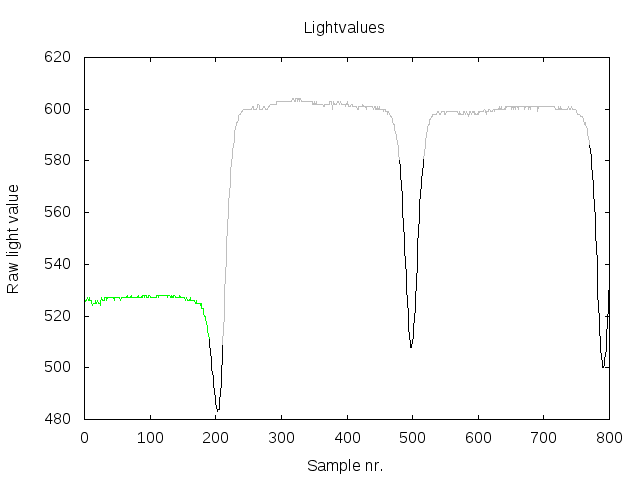
\includegraphics[scale=0.5]{../experiments/1prototype/results/gnuplot/GridAccuracyTilt_color.png}
  \caption{Light reading for a simple run from the base to the garage in a straight line (with the light sensor tilt)}
\end{figure}

Here
it is somewhat easier to tell green and black apart, so we will
experiment further with an angled light sensor.

Further testing reveals very inconsistent readings. From using the
datalogger with more experiments, we see that following a black line
reads values ranging from 425 to 540, with dips when we reach an
intersection. At these crossings, more black is seen, and so the light
value is lower than normal. Still we are able to see that this is not
white, which reads about 600, so we should be able to get the line
follower working. Another issue is that currently the light sensor is
too close to the line and it bumps into the solar panels sometimes. We
have to adjust its angle to move it further away from the center.

We only tested the ability to distinguish colors using the 3 cm above
method, we never got around to test line following capabilities. We then
tried going back to positioning the light sensor 5 cm above. In this
experiment, we had the robot drive straight forward, following a black
line. From the readings, it is easy to see when we are on a line, at an
intersection, at a solar panel and if it is
broken.
\begin{figure}[hbt]
  \centering
  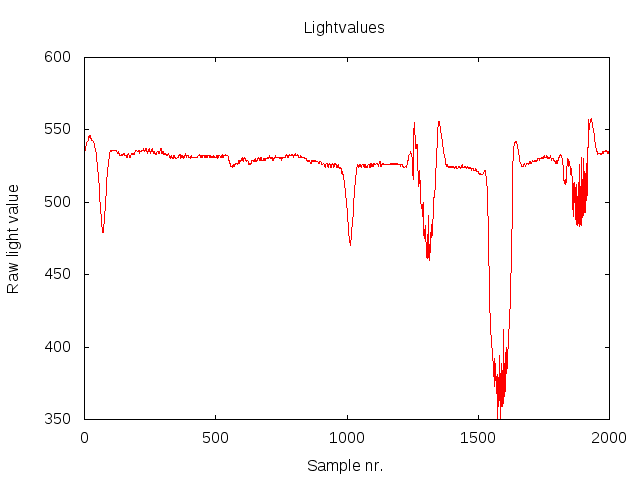
\includegraphics[scale=0.5]{../experiments/1prototype/results/gnuplot/GridAccuracyFollowBlack3cm.png}
  \caption{Light reading for a simple run, where the robot starts a the cross section inside the station and then follows the line out into space.}
\end{figure}

The
first two little spikes are from intersections, the next wider spike is
from a colored solar panel (notice the upward spikes from the gray area
before and just after the panel), then there's a huge spike from a black
solar panel, and finally another colored one.

Directions: We have assigned cardinal directions to the track in order
to more easily describe it. Moving out of the base is north, moving from
the green starting zone to the warehouse is west, and the remaining two
cardinal directions can be deduced from this. Driving ``north'': 602 and
``south'': 607, ``east'': 560 ``west'': 620. We get different readings
in different directions because of the windows in the building that are
facing ``west''. We also get different readings in the same direction
but at different positions on the track, because the light is not
uniformly distributed on the track. This makes it very difficult for us
to use line following in practice, and we may have to scrap the idea
entirely. The readings may get more precise if we move the light sensor
closer to the track, so we return to doing experiments at 3 cm distance.
Back at 3.4cm:

\subsubsection{Color distinguishing}
Clear distinction between
green and white, black and white, but the black line measured in the
white area reads about the same value as the green area. It will suffice
if we are clever about it, but it is not ideal.

\subsubsection{Line following:}

When following a line, it is very easy to see when we meet an
intersection. The light value drops about 50 units. Seeing a working
solar panel has about the same effect, but we will still be able to use
this to navigate the track. A broken solar panel is very easily
recognized, as the light value drops about 200. We are also able to tell
T sections from 4-way intersections, as these differ 20 units.

When moving in different directions on white, we read values between
570-630. This is quite a large range, but seeing as black is about 540,
it should not be an issue to tell them apart.

After initial testing of the line follower, we found that the single
light sensor is not accurate enough, so we will be using two light
sensors. We will position the two sensors at a height of 3.4 cm above
the surface, 4 cm apart so there is room for a line between them.\\Now
we have the issue of two light sensors reporting different values on the
same surface. There is roughly a 50 unit difference, so we need to make
a mapping so that they are equal. If this is anything like the week we
used two sound sensors, this will not be an easy task. The mapping could
be non-linear and impossible to predict.\\We appear to have some success
calibrating the two sensors by subtracting their difference from the
higher value, and thus equalizing them. This is assuming there is a
constant offset, which is unlikely, but we did manage to get the vehicle
to follow a line using this approach.

\subsection{Conclusion}

Due to all of there sources of disturbance (lighting in the room,
difference between sensors, inaccuracy due to distance from the track),
we conclude that it is unfeasible to use the solar panel manipulation
approach we decided on last time; lifting solar panels using some sort
of lifting mechanism. We simply cannot get the desired accuracy of 2 mm
on the line follower.\\We have to postpone the solar panel manipulation
mechanism until next meeting, so we did not reach the goal for today. We
decided to continue with the mechanism that pushes a solar panel aside
into a slot for carrying, which we will build next time hopefully.
